\chapter{Implementación}

En este capitulo se presentá la implementación de cada uno de los componentes del sistema, tanto de software como de hardware.

\section{Controladores}

Una de las decisiones de diseño más importantes fue la de escoger un sistema de control distribuido, de esta forma los controladores son modulares e idénticos entre sí. Básicamente se compone de una unidad de procesamiento, el microcontrolador, y la sección de potencia, compuesta por el puente H.

\subsection{Integración de hardware}

El microcontrolador corresponde al Infineon XMC4800, pues posee un conjunto de periféricos ideal para el tipo de aplicación requerida. Para reducir el tiempo de desarrollo y simplificar la implmentación se usó como elemento base la placa de desarrollo del microcontrolador y puente H, de esta forma se diseñó una PCB para el montaje de las placas de desarrollo usando una estructura por pisos (\textit{stackable}).

\subsubsection{PCB}

Habiendo escogido un diseño basado en placas de desarrollo, la PCB tiene el papel de integrar eléctrica y mecánicamente los distintos componentes presentados en la Tabla \ref{cap4_componentes_pcb}.

\begin{table}[]
\centering
\label{cap4_componentes_pcb}
\begin{tabular}{|l|l|}
\hline
\textbf{Elemento}                                    & \textbf{Tipo de montaje}            \\ \hline
Montaje para placa de desarrollo del microcontrolador XMC4800     & THT Pin header \SI{0,1}{\inchQ}     \\ \hline
MOntaje para puente H basado en BTN8982TA                         & THT Pin header \SI{0,1}{\inchQ}     \\ \hline
Sensor de corriente TLI4970                          & SMT                                 \\ \hline
Conector DB9                                         & THT                                 \\ \hline
Conectores de poder                                  & THT                                 \\ \hline
Otros Elementos pasivos (resistencias y capacitores) & THT                                 \\ \hline
\end{tabular}
\caption{Componentes del PCB.}
\end{table}

Dada que existen componentes SMT (\textit{Surface Mount Technology}) y THT (\textit{Through Hole Technology}), se escoje un diseño usando dos capas. En la parte superior se dispone el montaje para la placa de desarrollo XMC4800, sensor de corriente y conector DB9 para el motor, en lado posterior se ubica el montaje para el puente H.

Para el diseño de los circuitos equemáticos y PCB (Ver \ref{anexo_esq}) se usó el software Eagle\textregistered 7.5.0, que es un estándar para proyectos de baja complejidad y los fabricantes proveen librarías de sus productos para éste software. El sensor de corriente TLI4970 usa un \textit{footprint} especial \texttt{PG-TISON-8-1} que no se encuentra en la librería estandar del software, por lo que tuvo que ser diseñado.

Un hecho importante a la hora del diseño es considerar las limitaciones la máquinaria disponible para la construcción, así para la construcción del PCB se cuenta con una máquina de protipado LPKF\textregistered,  cuya principal limitante es que que no realiza vias, así el diseño intenta minizar el uso de vias. Un elemento de diseño escencial en los PCB, corresponde a considerar los flujos de corriente y sus retornos, pues es el parametro principal al momento de considerar el ancho de las pistas y ubicación de componentes, en este sentido todas las pistas encargadas de transportar la corriente hacía el motor son un ancho mayor y todos los componentes asociados, como el sensor de corriente, se encuentran ubicados de forma próxima.

Para ejecutar el diseño se necesario hacer uso de un software CAM especializado en el cual se importan los diseños generados en Eagle\textregistered.  Para soldar el sensor de corriente TLI4970 es necesario emplear una soldadora BGA para soldar el integrado a la PCB, pues los puntos de soldadura (\textit{pads}) se encuentran por debajo del integrado. La Figura \ref{cap4_pcb} muestra la PCB obtenida desde la máquina LPKF\textregistered.


\begin{figure}[H]
  \centering
  \begin{subfigure}[b]{0.35\textwidth}
    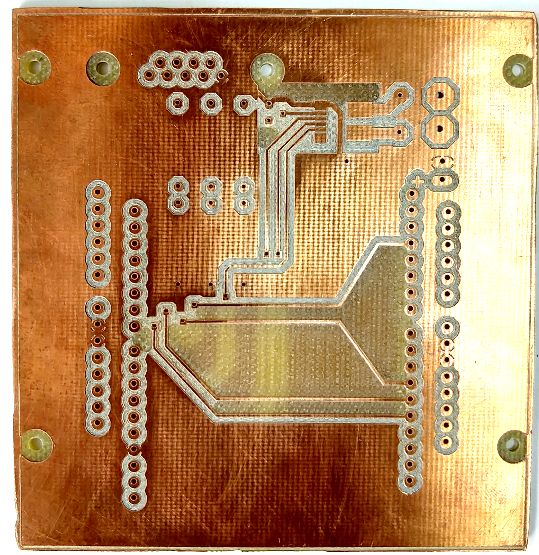
\includegraphics[width=0.9\textwidth]{img/cap4/top_pcb}
    \caption{Cara superior (\textit{top}).}
    \label{cap4_top_pcb}
  \end{subfigure}%
  ~
  \begin{subfigure}[b]{0.35\textwidth}
    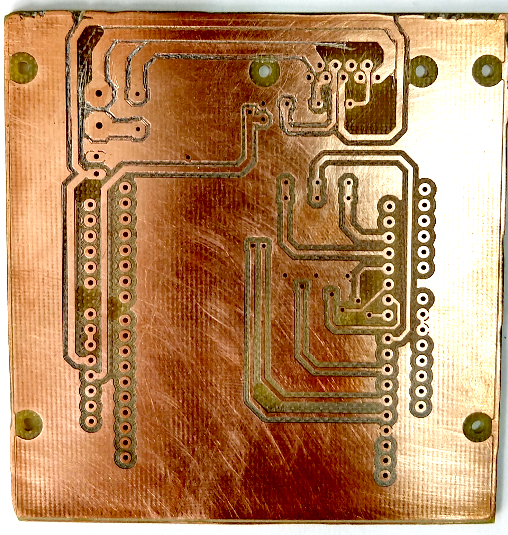
\includegraphics[width=0.9\textwidth]{img/cap4/bottom_pcb}
    \caption{Cara inferior (\textit{bottom}).}
    \label{cap4_bottom_pcb}
    \end{subfigure}
  \caption{PCB fabricada con LPKF\textregistered.}
  \label{cap4_pcb}
\end{figure}

Una vez montados todos los componenetes del PCB se obtiene lo mostrado en la Figura \ref{cap4_controlador_completo}, la alimentación del microcontrolador se dispone por un costado, mientras que la alimentación del puente H se encuentra en la parte posterior de la placa, los conectores RJ-45 para la red EtherCAT se encuentran juntos para facilitar la conexión \textit{daisy chain} y el conector DB9 para los motores del robot Scorbot se encuentra en un extremo de la placa. 

\begin{figure}[H]
  \centering
  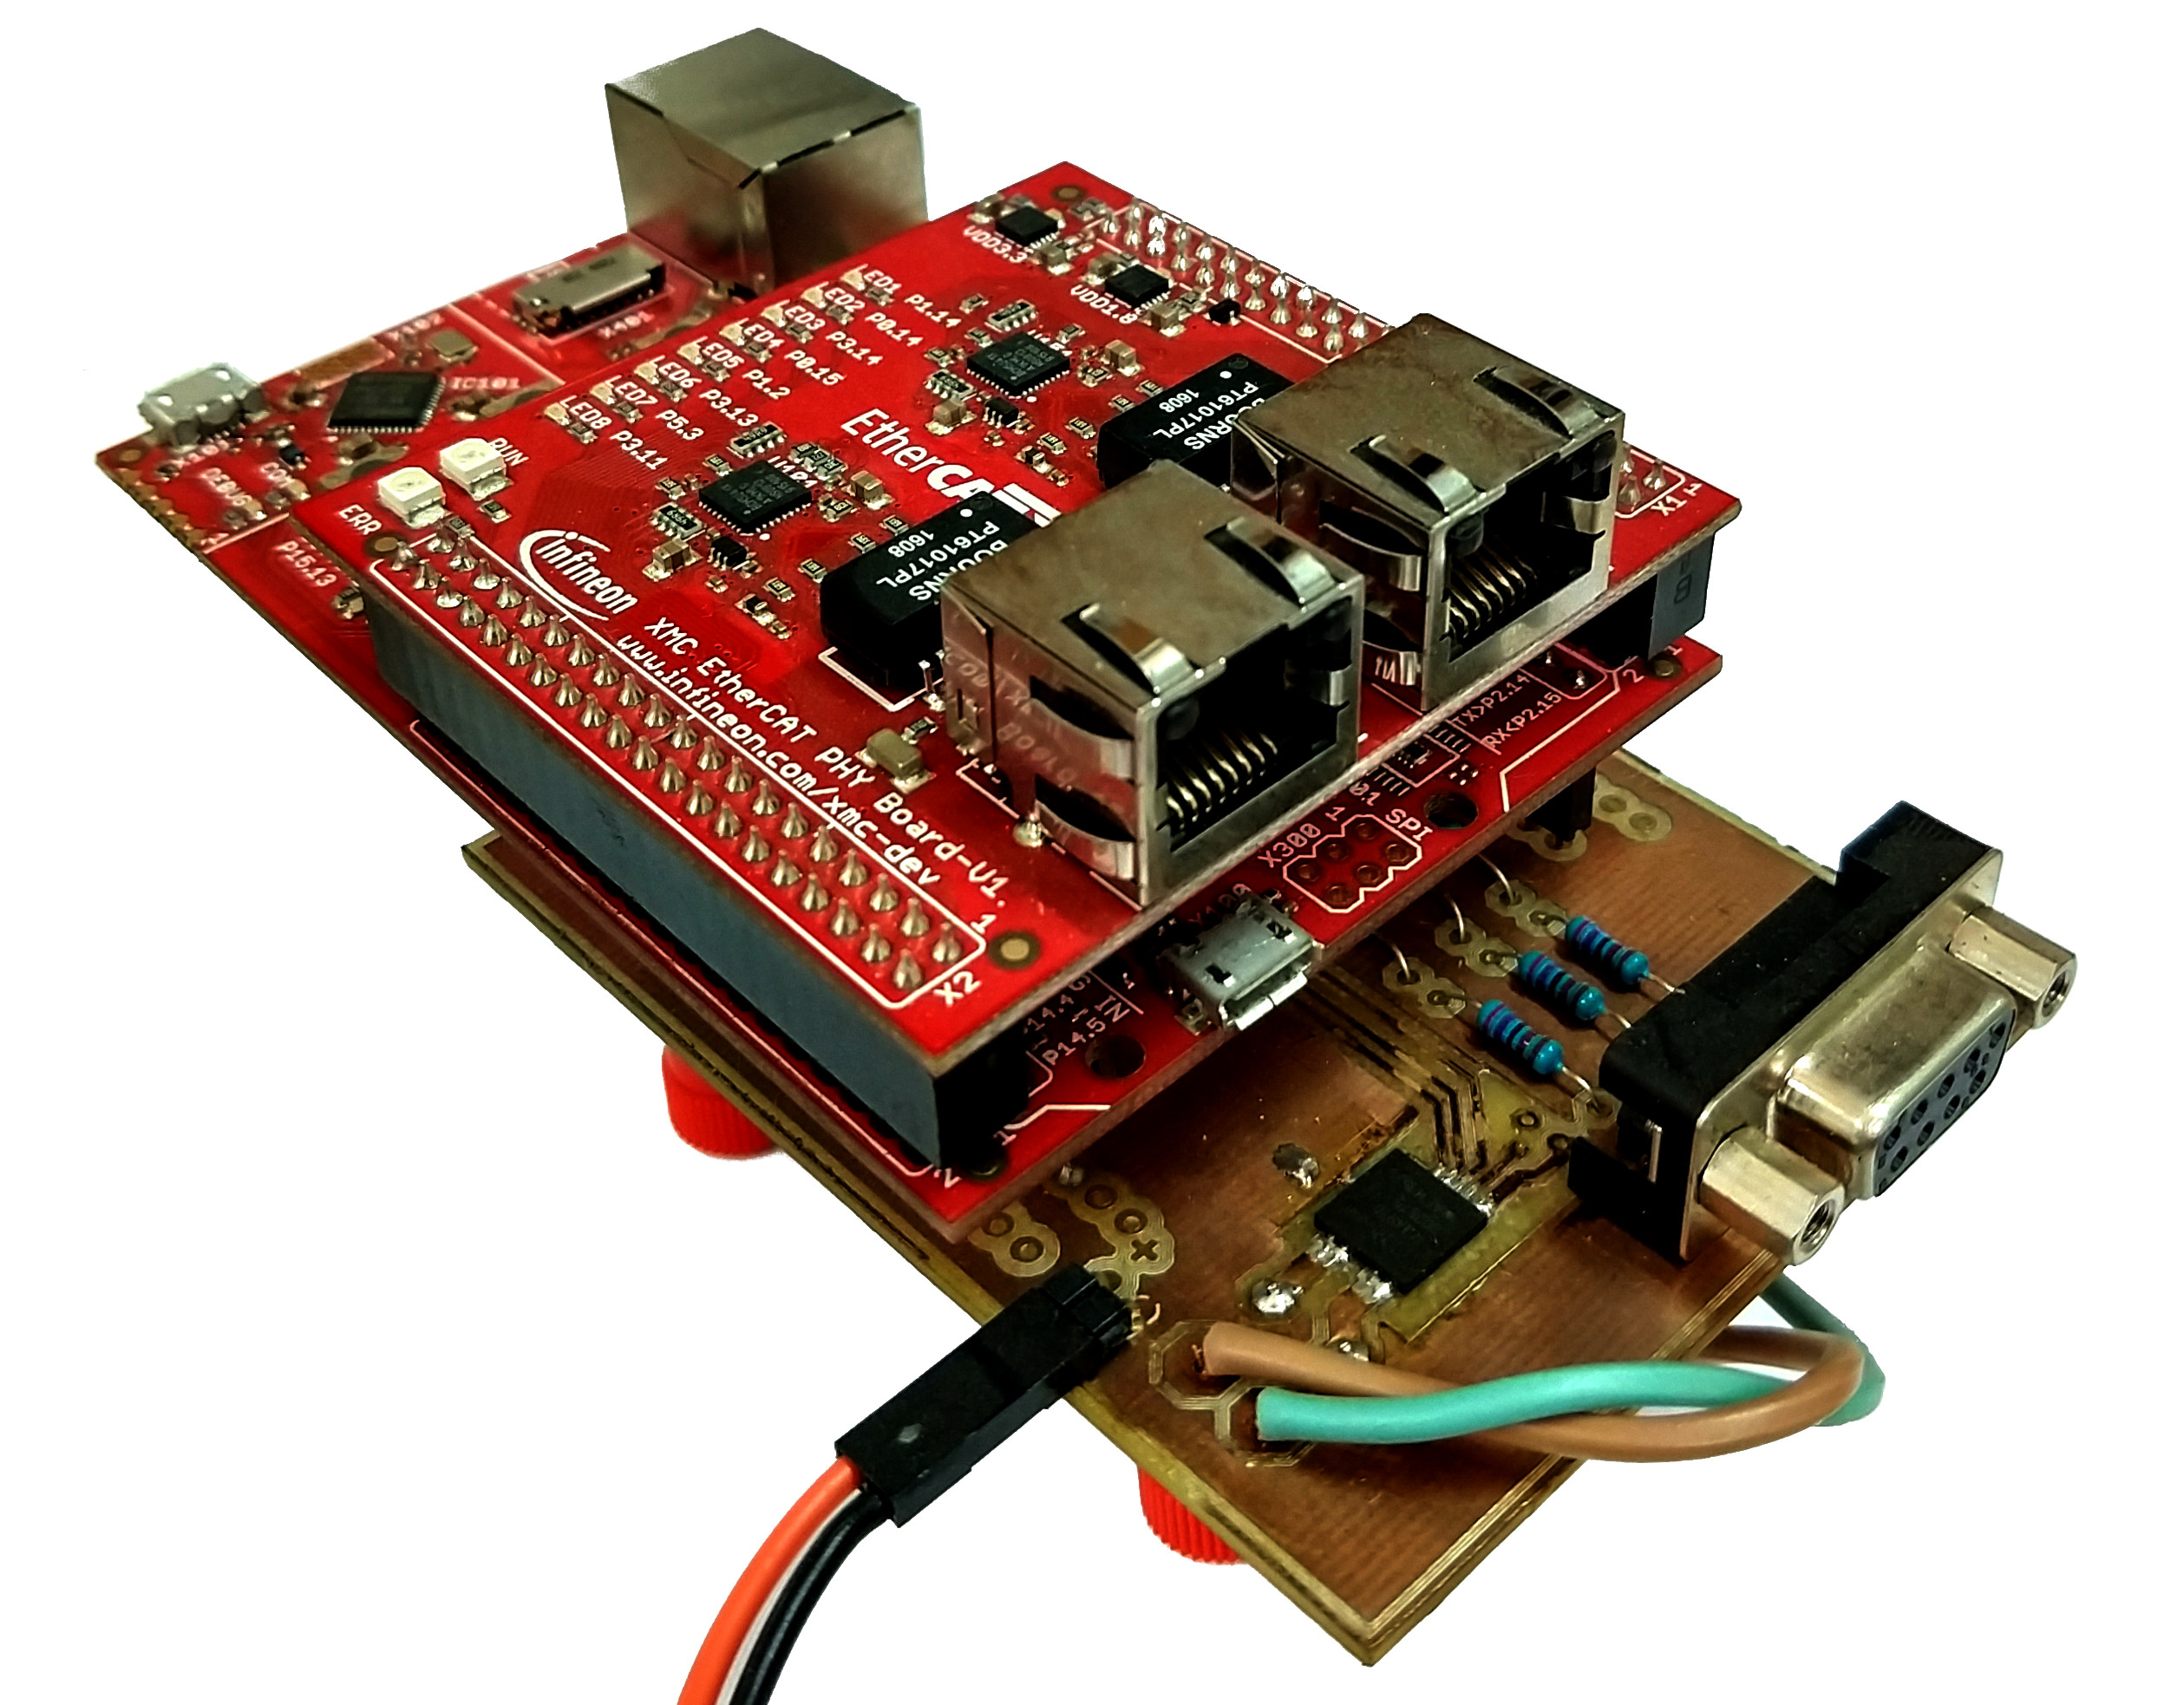
\includegraphics[width=0.5\textwidth]{img/cap4/board}
  \caption{Controlador completo montado.}
  \label{cap4_controlador_completo}
\end{figure}

\section{Bus de campo}

El bus de campo EtherCAT se conecta con una topología \textit{Daisy chain} usando cables de par trenzado con conectores RJ45. Dado que EtherCAT usa la capa física y de enlace de datos de Ethernet, se puede emplear el mismo cableado usado para redes de computación.

De esta forma se configuró un montaje para disponer de todos los controladores de forma alineada, esta configuración se muestra en la Figura \ref{cap4_montaje}


\begin{figure}[H]
  \centering
  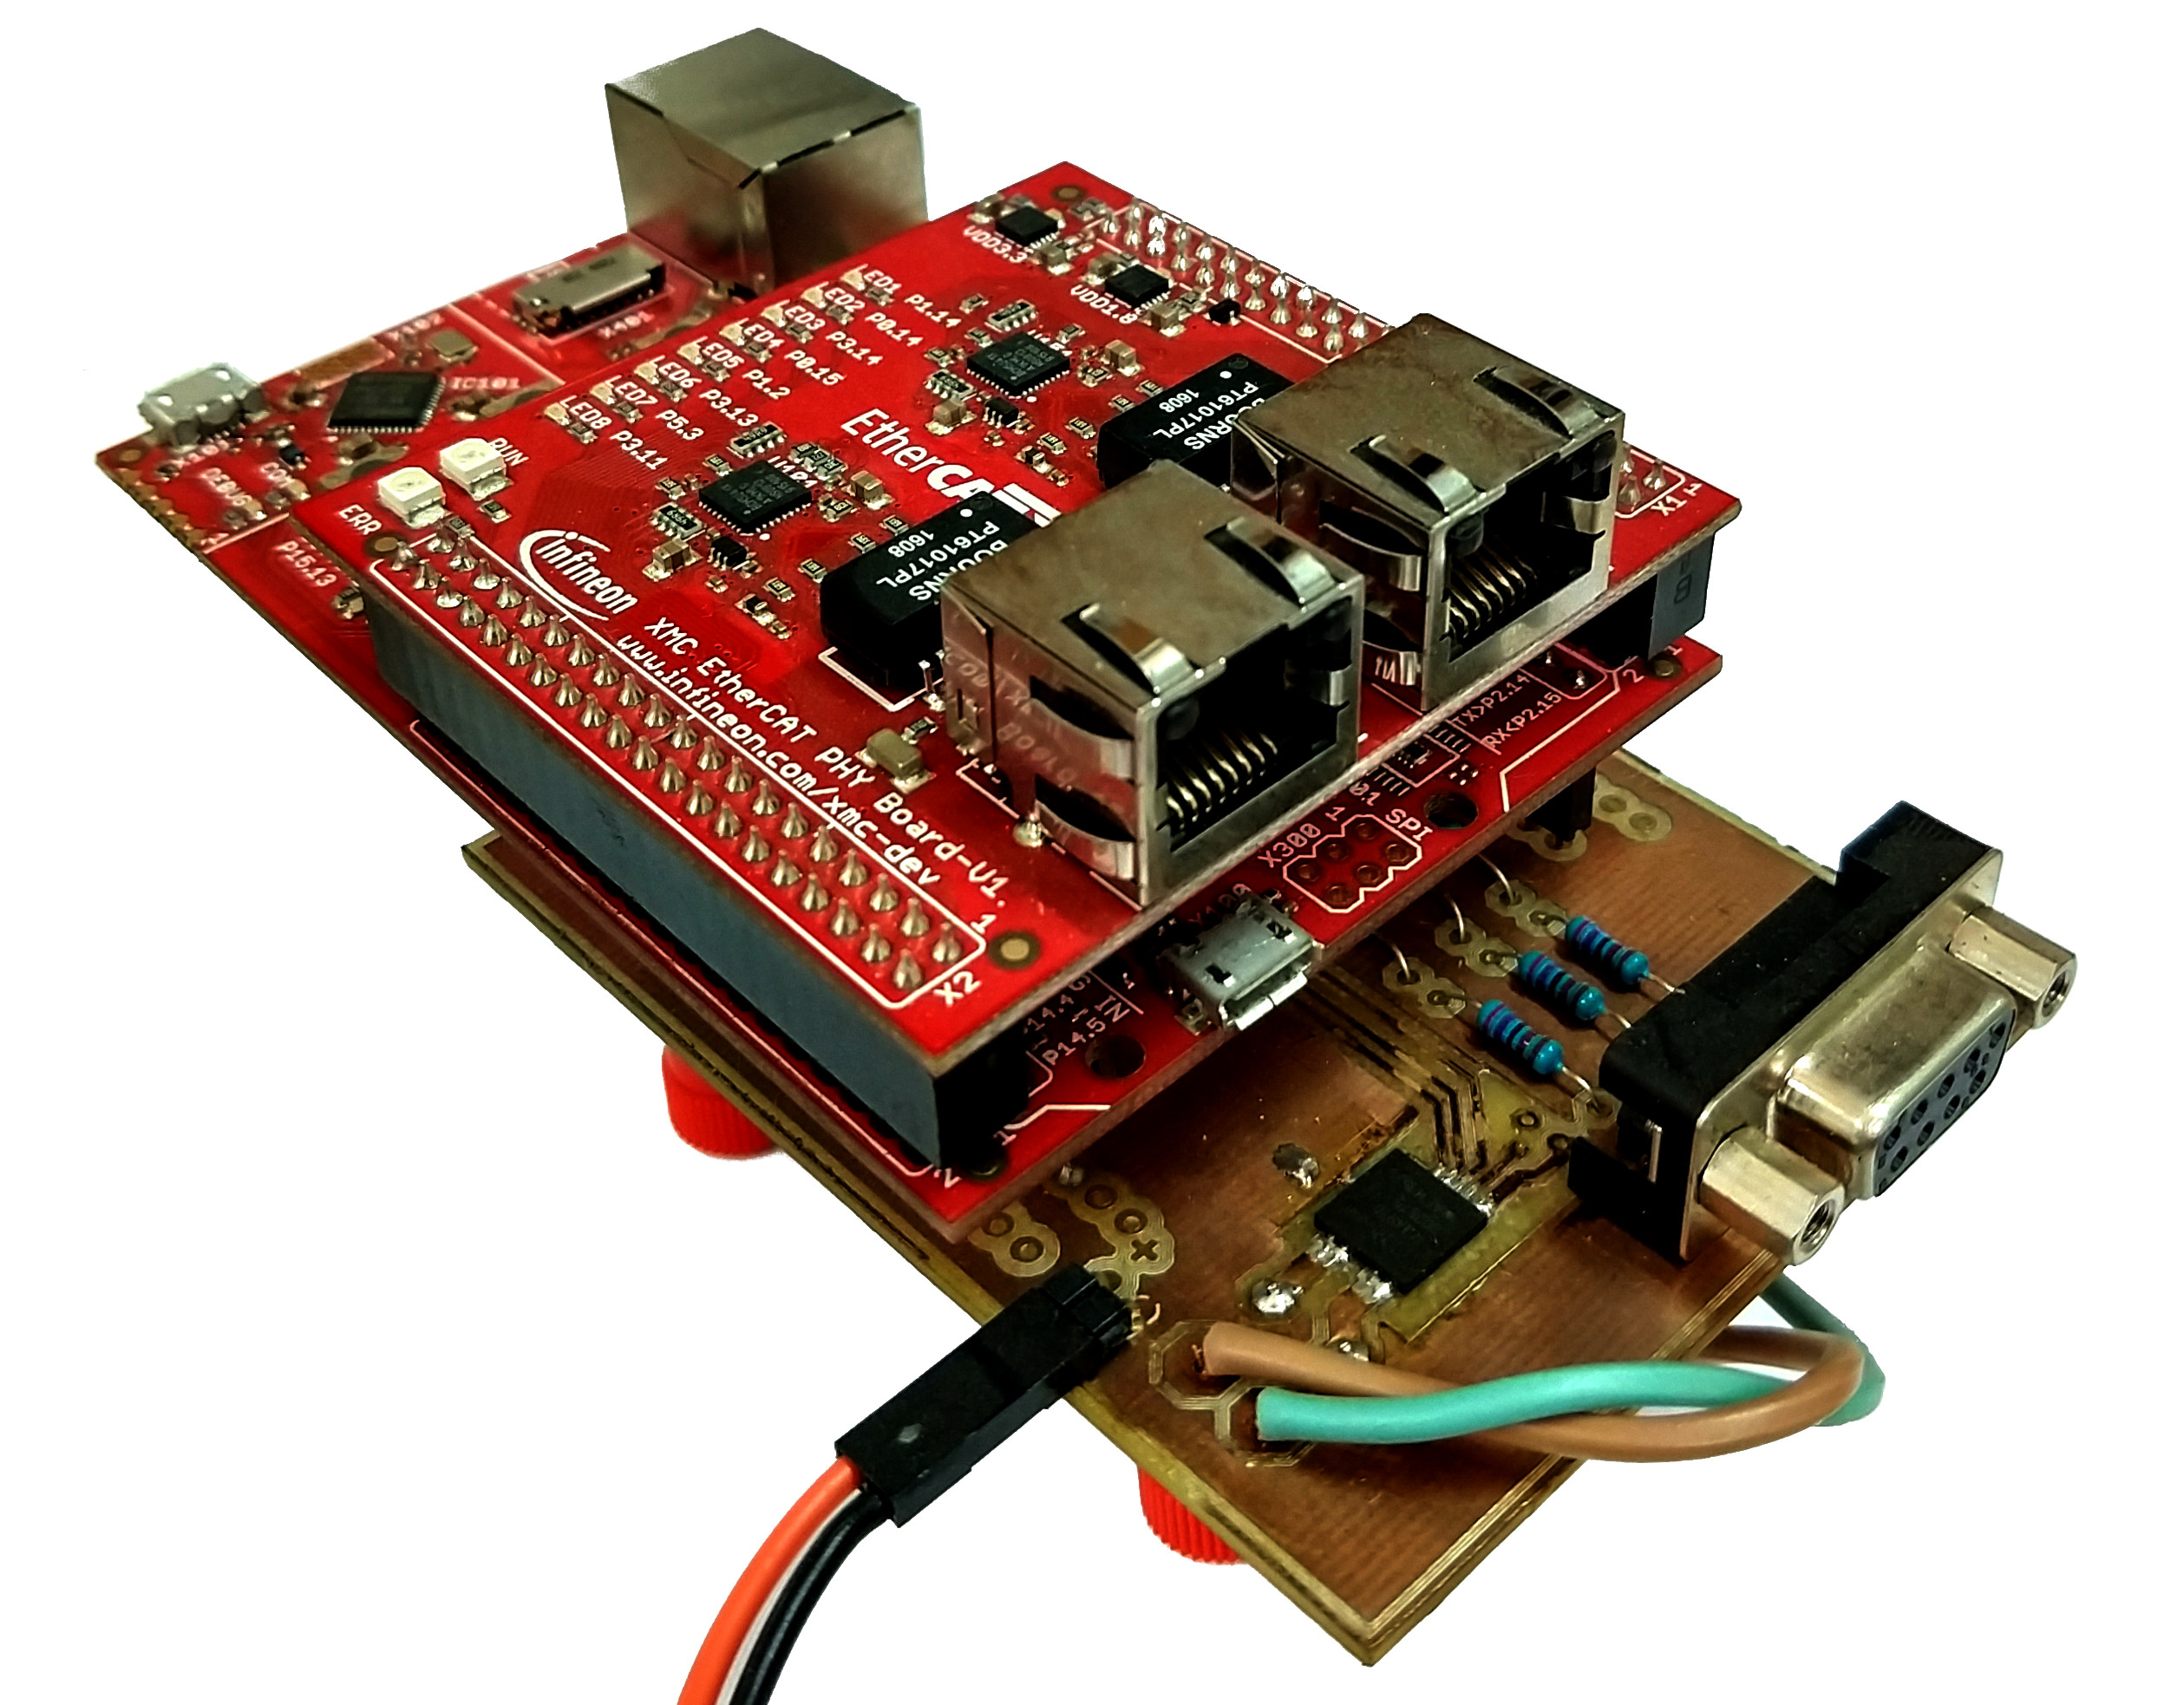
\includegraphics[width=0.5\textwidth]{img/cap4/board}
  \caption{Montaje de controladores.}
  \label{cap4_montaje}
\end{figure}

\section{Software}

En esta sección se describirá el software desarrollado, esta compuesto por dos grandes módulos: software embebido que se ejecuta en el microcontrolador (\textit{firmware}) y el conjunto de programas que se ejecutan desde el computador usando el framework ROS.

\subsection{Firmware}

El firmware corresponde al software que se ejecuta en el microcontrolador, su principal tarea es la ejecución del ciclo de control. El Firmware se implementó en lenguaje C, haciendo uso de librerías del fabricante para la configuración y control de perifericos. La Figura \ref{cap4_scorbot_firmware} muestra de forma gráfica los distintos elementos del \textit{firmware}.

\begin{figure}[ht]
  \centering
  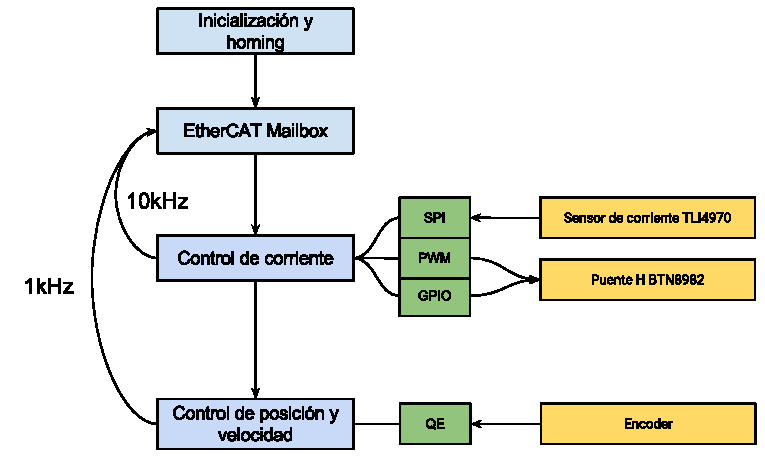
\includegraphics[width=0.6\textwidth]{img/cap4/scorbot_firmware.pdf}
  \caption{Diagrama de funcionamiento del firmware.}
  \label{cap4_scorbot_firmware}
\end{figure}


\subsubsection{Inicialización}

Corresponde a la primer bloque de código ejecutado, aquí se configuran todos los periferios utilizados, por ejemplo: configuración de I/O, frecuencia y modo del módulo SPI, frecuencia y resolución del timer de la unidad de PWM.

\subsubsection{\textit{Homing}}

Así se denomina a la determinación de la posición inicial de cada articulación del robot Scorbot (\textit{home position}). Dado que el robot Scorbot solo cuenta con encoders incrementales, el procedimiento de \textit{homing} debe realizarce cada vez que se inicie el robot.

El robot cuenta con interruptores que permiten determinar la posición central de cada articulación, lamentablemente debido al estado del robot, estos interruptores se encuentran en mal estado, por lo que se decidio considerar la posición fisica del robot como posición \textit{home} al iniciar el robot. Esto se traduce en que el operador debe posicionar el robot en la posición \textit{home} al momento de encender el robot.

\subsubsection{EtherCAT mailbox}

El protocolo EtherCAT a nivel de \textit{firmware} usa el patrón \textit{mailbox}, de esta forma el ciclo de control obtiene una estructura de datos actualizada en cada iteración y escribe en otra estructura de datos el estado del sistema al final del ciclo. Es tarea del EtherCAT SSC que estas estructuras de datos se mantengan actualizadas y esten disponibles para el dispositivo maestro.
 
\subsubsection{Controladores}

El controlador digital presentado en la sección \ref{cap3_controladores} se implementó en lenguaje C usando la transformada directa II.

%https://www.keil.com/pack/doc/CMSIS/DSP/html/group__BiquadCascadeDF2T.html

\subsection{ROS}

Como se monstró en el capitulo pasado, su utilizó ROS como framework para realizar la integración. Los dispositivos de hardware, el robot Scorbot y el dispotivo háptico Phantom, cuentan con su \textit{nodo driver} que permiten la integración con el ecosistema ROS.

Se entiende por \textit{nodo driver} o ROS \textit{wrapper}, a una aplicación que actua como puente entre un dispositivo fisico y su representación en ROS, permitiendo interactuar de forma transparente con el dispositivo mediante el uso tópicos y servicios. Usualmente el \textit{nodo driver} hace uso de librerías proveidas por el fabricante o terceros para el manejo protocolos especificos del dispositivo. Por ejemplo, las siguientes aplicaciones cumplen esta función:

\begin{itemize}

\item \textit{ROSARIA}\cite{rosaria}: corresponde a una aplicación construido usando la librería \textit{Adept MobileRobots Robotics Interface for Applications} (ARIA), permite el control de robots móviles de las compañias Adept MobileRobots, MobileRobots Inc., y ActivMedia, por ejemplo el Pioneer 3-DX y 3-AT.

\item \textit{kinova-ros}\cite{kinova}: Es el driver oficial ofrecido por Kinova robotics para el uso de los robot manipuladores Jaco y Mico.

\end{itemize}

\subsubsection{Integración del robot Scorbot}

En esta sección se describirá la función de cada uno de los nodos que integran el software desarrollado para el control del robot Scorbot.

\begin{figure}[ht]
  \centering
  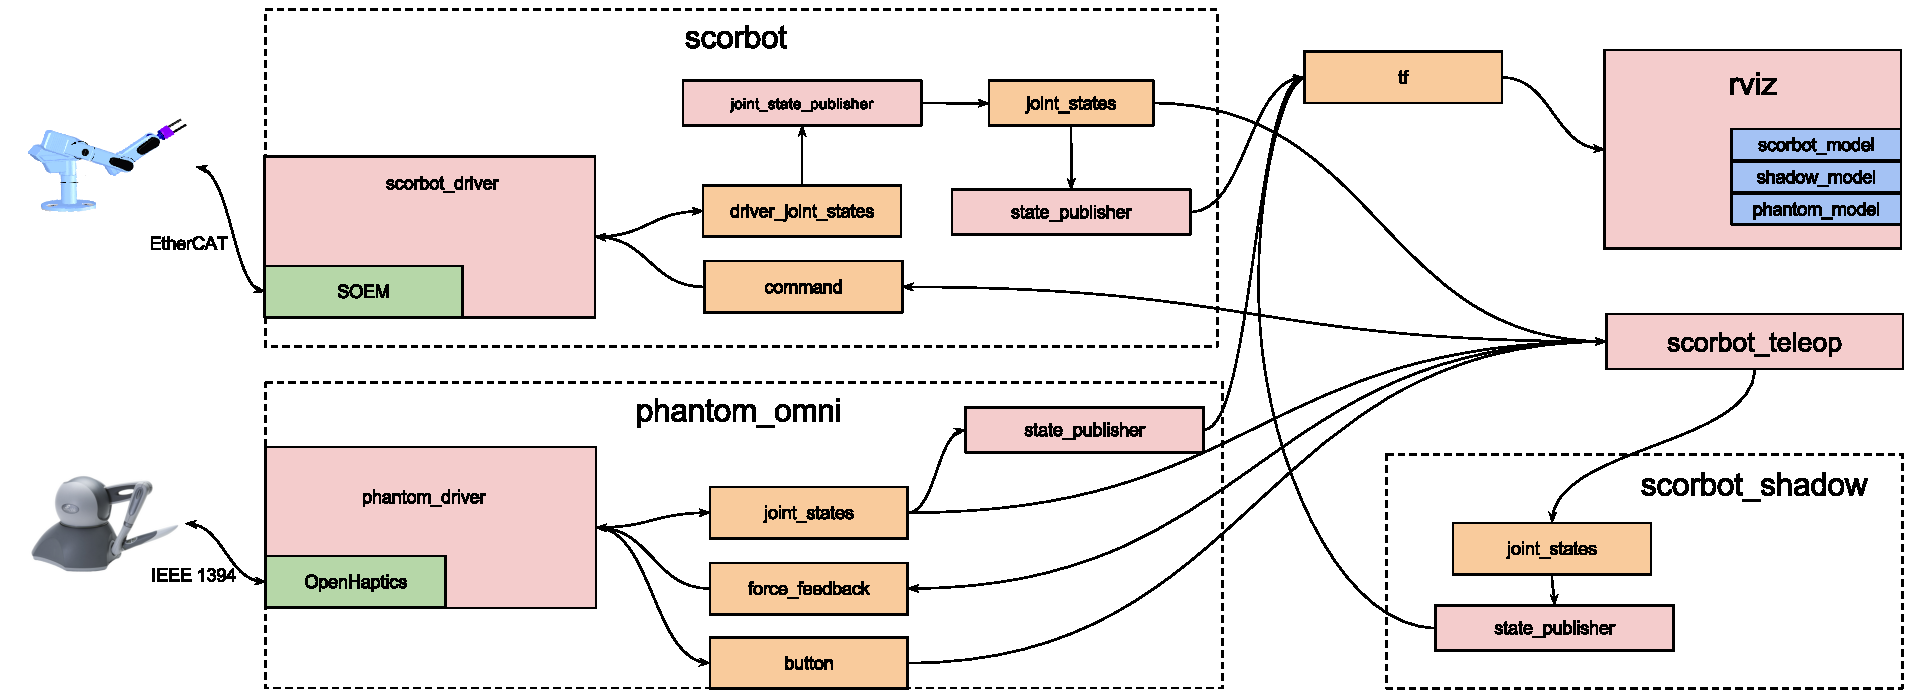
\includegraphics[width=\textwidth]{img/cap4/scorbot_software.pdf}
  \caption{Diagrama de nodos y tópicos de la aplicación.}
  \label{cap4_scorbot_software}
\end{figure}

\begin{description}

\item[\texttt{scorbot\_driver}] Corresponde al \textit{nodo driver} se integra con la librería SOEM \cite{soem} para la comunicación EtherCAT. Dado que este nodo ejecuta un ciclo de control, se consideraron una serie de requerimientos, muchos de ellos básicos para software de ejecución en tiempo real:

\begin{itemize}
\item Separación de hilos de ejecución, todas las tareas realacionadas con actualización de datos en el bus de control se realiza en un hilo independiente (\textit{control thread}) a las comunicaciones con el framework ROS (ROS \textit{thread}).
\item La comunicación entre el  \textit{control thread} y el ROS \textit{thread} se realiza usando estructuras de datos no bloqueantes.
\item La memoria utilizada por el hilo de control queda fija luego de la inicialización, de esta forma no se hacen llamados al sistema para pedir o liberar memoria.
\end{itemize}

SOEM mapea en memoria los dispositivos, es decir, desde el la aplicación master se tiene acceso a un buffer de memoria que permite leer y escribir en los dispositivos esclavos. Para obtener los datos manipulables, se debe usar la misma estructura de datos que usa el dispositivo esclavo para representar la información. \texttt{setpoint\_t} es la estructura usada como referenca (\textit{set point}), miestras que \texttt{joint\_data\_t} es la información del estado del controlador. Estas estructuras estan contenidas en un archivo de cabezera generado por el SSC, su modificación debe realizarse de forma cuidadosa, pues se pueden obtener errores de representación. El Código fuente \ref{cap4_estructuras} muestra la composición de ambas estructuras, notar el uso de la instrucción \texttt{PACKED}, que indica al compilador no añadir bytes entre los elementos de la estructura, de esta forma todos los elementos estan contiguos en memoria.

\begin{lstlisting}[language=C,style=csstyle, caption=Estructuras de datos usadas para mapear datos de dispositivos esclavos, label=cap4_estructuras]
typedef struct PACKED {
    uint16_t controlRegA;
    uint16_t controlRegB;
    int16_t  currentRef;
    int16_t currentLim;
    uint16_t pidCurrentKp;
    uint16_t pidCurrentKi;
    uint16_t pidCurrentKd;
} setpoint_t;

typedef struct PACKED {
    int16_t encPosition;
    int16_t encSpeed;
    int16_t current;
    uint16_t limits;
} joint_data_t;
\end{lstlisting}

Luego de realizar el mapeo en memoria, se creó la clase \texttt{ScorbotJointDriver}, encargada de representar cada controlador. Posee metodos para modificar la referencia y obtener el estado del controlador. Todos los controladores se agrupan en la clase \texttt{ScorbotHardwareInterface}, la cual abstrae las funciones del robót manipulador, como enviar una referencia a todas las articulaciones y detener todos los controladores. Es también encargada de ejecutar el ciclo de actualización de todos los controladores, este ciclo se ejecuta a \SI{1}{\kilo\hertz}.

ROS posee el paquete \texttt{ros\_control}, cuya función es facilitar la integración de dispositivos de control en ROS. De esta forma la clase \texttt{ScorbotHardwareInterface} hereda de \texttt{hardware\_interface::RobotHW} permitiendo la integración con \texttt{ros\_control}. El principal elemento utilizado de \texttt{ros\_control} correponde al \texttt{cotroller\_manager} una clase encargada de la comunicación entre \texttt{hardware\_interface::RobotHW} y tópicos ROS usando estructuras no bloqueantes en un hilo de ejecución independiente.

\begin{figure}[ht]
  \centering
  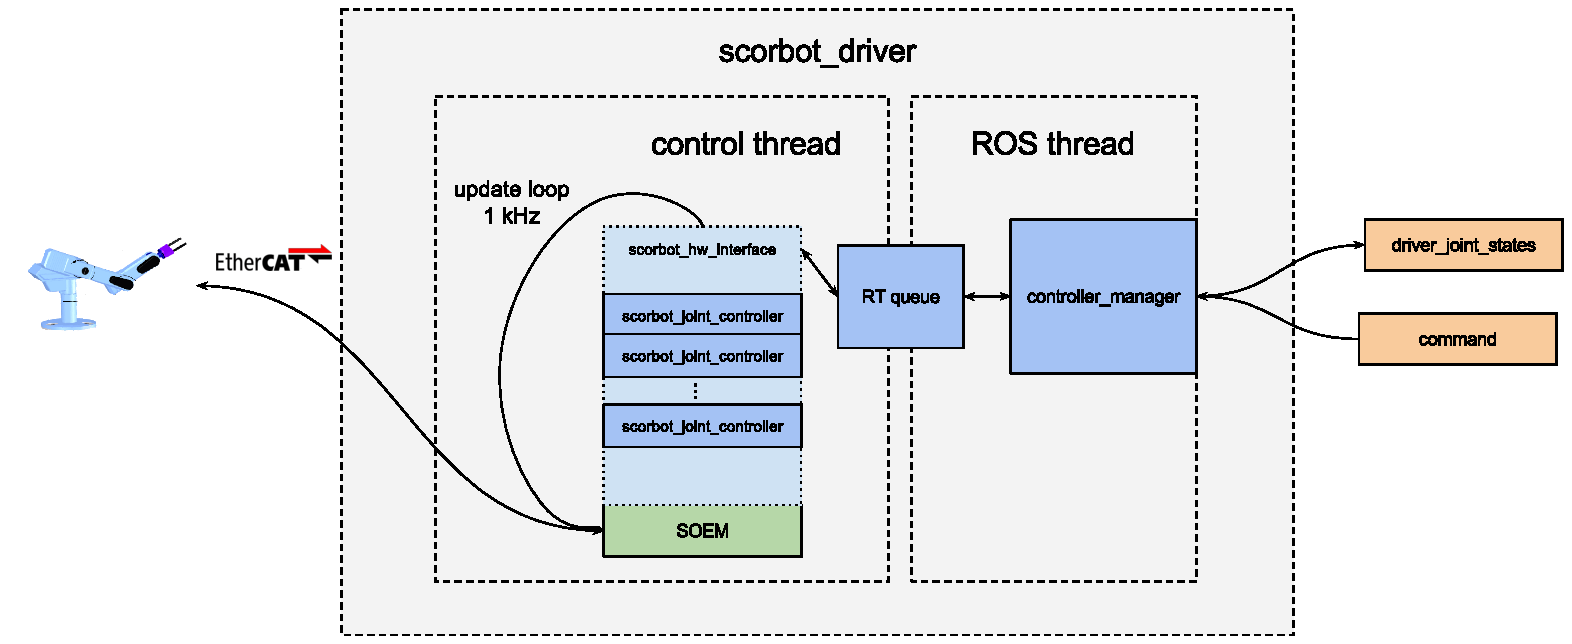
\includegraphics[width=\textwidth]{img/cap4/scorbot_driver.pdf}
  \caption{Diagrama del nodo \texttt{scorbot\_driver}.}
  \label{cap4_scorbot_driver}
\end{figure}

La Figura \ref{cap4_scorbot_driver} muestra la estructura del nodo \texttt{scorbot\_driver} como se ha señalado anteriormente. Como se ha mensionado anteriormente, es el \texttt{controller\_manager} quien se encarga de la comunicación con ROS, usando distintos tópicos:

\begin{itemize}

\item \texttt{driver\_joint\_states}: Contiene la información sobre el estado de cada articulación: posición, velocidad, aceleración y tiempo. Usa el mensaje  \texttt{sensor\_msgs/JointState[]}.

\item  \texttt{command}: Se usa para obtener la referencia de posición que será enviada a los controladores, se usa el mensaje \texttt{std\_msgs/Float64[]}.
 
\end{itemize}



\item[\texttt{joint\_state\_publisher}] Corresponde a un nodo estándar de ROS, cuya función es obtener los estados de las articulaciones de distintas fuentes (tópicos) y publicarlos de forma conjunta, completando el estado de todas las articulaciones dependiendo de la descripción del robot (URDF).

\item[\texttt{robot\_state\_publisher}] Corresponde a un nodo estándar de ROS, es el encargado de tomar la información de las articulaciones del robot y publicar el árbol de transformadas de cada uno de los enlaces del robot basado en la descripción del robot (URDF), es decir, ejecuta la cinemática directa del robot. Esta información de las transformadas es publicada en el tópico \texttt{/tf}.

\end{description}


\subsubsection{Modelo URDF}

El \textit{Unified Robot Description Format} (URDF) es un formato basado en XML (\textit{Extensible Markup Language}), corresponde al estandar para la representación de robots en el framework ROS. Este archivo de describe las propiedades cinemáticas y dinámicas del robot, básicamente se especifican las características de los enlaces (\textit{links}) y articulaciones (\textit{joints}).

El formato URDF usa una estructura de arbol para representar los distintos elementos del robot, esto impide la representación de mecanismos cerrados o \textit{loops}, sin embargo la estructura del robot Scorbot corresponde a una simple cadena cinemática. Escribir URDF directamente puede ser una tarea monotona y difícil de depurar, por lo que para crear el URDF del robot Scorot se usó una aproximación gráfica a partir de un modelo CAD.

El modelo CAD se creó usando el software de modelamiento SolidWorks 2014 \textregistered, junto con el \textit{plugin} \texttt{sw\_urdf\_exporter} \cite{sw_urdf}, que permite generar el modelo URDF y archivos STL que representan los \textit{links} del robot. La Figura \ref{cap4_scorbot_cad} muestra el modelo del robot Scorbot en el software CAD en la posición \textit{home}.

\begin{figure}[H]
  \centering
  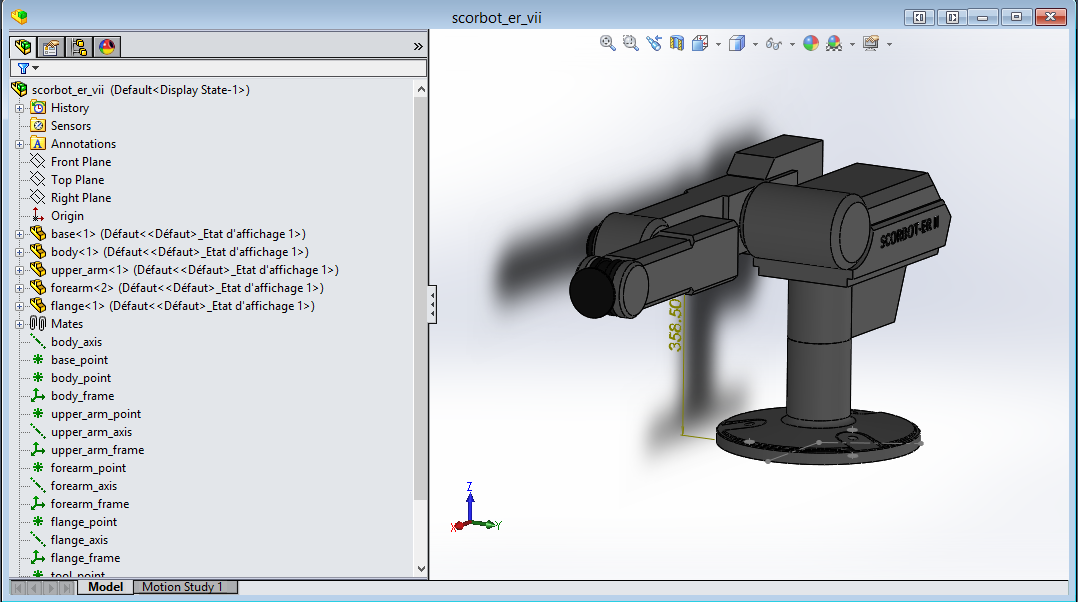
\includegraphics[width=0.8\textwidth]{img/cap4/cad_solidworks.PNG}
  \caption{Modelo del robot Scorbot en SolidWorks 2014 \textregistered.}
  \label{cap4_scorbot_cad}
\end{figure}

Luego de ajustar los puntos de referencia y ejes de cada una de las articulaciones se preocede con exportar el modelo hacia el formato URDF. Una vez exportado, se realizan algunos ajustes manuales al modelo, como corrección de los ángulos limite, posición por defecto y color de los \textit{links}. Con los distintos elementos se contruye el paquete \texttt{scorbot\_description}, que contiene el URDF, archivos STL y utilidades básicas de visualización. La Figura \ref{cap4_scorbot_rviz} muestra el modelo URDF del robot Scorbot en el visualizador \textit{RViz} de ROS.

\begin{figure}[H]
  \centering
  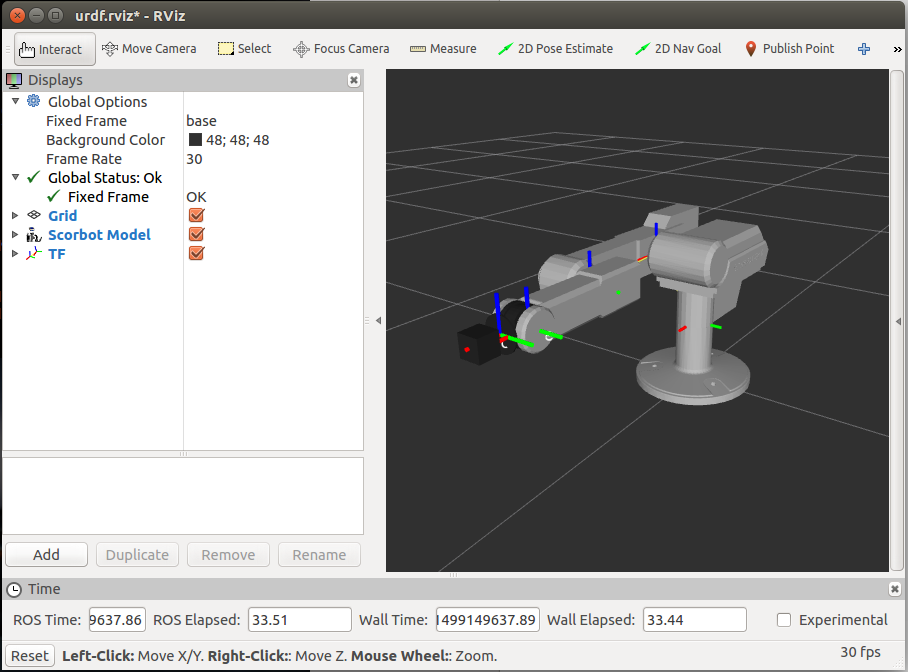
\includegraphics[width=0.8\textwidth]{img/cap4/scorbot_rviz.png}
  \caption{Modelo del robot Scorbot en \textit{RViz}.}
  \label{cap4_scorbot_rviz}
\end{figure}

\subsubsection{Integración de la interfaz Phantom Omni}

En esta sección se describirá la integración del dispositivo Phantom Omni en ROS. En este caso se hace uso del paquete \textit{phantom\_omni}\cite{phantom_git}, que contiene el ROS wrapper y URDF. La integración del Phantom Omni en ROS es similar a la realizada con el robot Scorbot, pues cuenta con el  ROS wrapper y los nodos \texttt{robot\_state\_publisher} y  \texttt{joint\_state\_publisher}, que cumplen la misma función descrita anteriormente, salvo que actúan sobre el estado del Phantom Omni.

\texttt{phantom\_driver} Corresponde al \textit{nodo driver} se integra con la librería OpenHaptics para la comunicación con dispositivo Phantom Omni a través de FireWire. Provee los siguientes tópicos:

\begin{itemize}
\item \texttt{joint\_states}: Información sobre el estado de las articulaciones usando el mensaje \\ \texttt{sensor\_msgs/JointState[]}.

\item \texttt{button}: Información sobre el estado de los botones del stylus del Phantom Omni, usando el mensaje \texttt{omni\_msgs/OmniButtonEvent}.

\item \texttt{force\_feedback}: El nodo se suscribe a éste tópico, al publicar en él el dispositivo aplica un par sobre las articulaciones actuadas.
\end{itemize}

Todos los tópicos del \texttt{phantom\_driver} se ejecutan a una frecuencia de \SI{100}{\hertz}, esto asegura que la referencia y retroalimentación hacia el operador sea adecuada, en terminos de retardo.


\subsubsection{Teleoperación}\label{cap4_teleoperacion}

La aplicación encargada de la teleoperación debe, básicamente, conectar el robot Scorbot con la interfaz háptica Phantom Omni, por conectar se entiende que la aplicación realiza el mapeo de las articulaciones del Phantom Omni hacia las articulaciones del Scorbot y entrega retroalimentación usando el Phantom Omni. Esta tarea es realizada por el nodo \texttt{scorbot\_teleop}.

El nodo \texttt{scorbot\_teleop} no controla directamente al robot Scorbot, si no que a un robot virtual, denominado Scorbot \textit{shadow}, esta representación almacena la posición deseada para el robot. Uno de los botones del \textit{stylus} del Phantom Omni actúa como gatillo, enviando la referencia es enviada al robot. Si el usuario mantiene el botón presionado, el software enviará de manera continua (\SI{100}{\hertz}) la referencia al robot.

\begin{figure}[H]
  \centering
  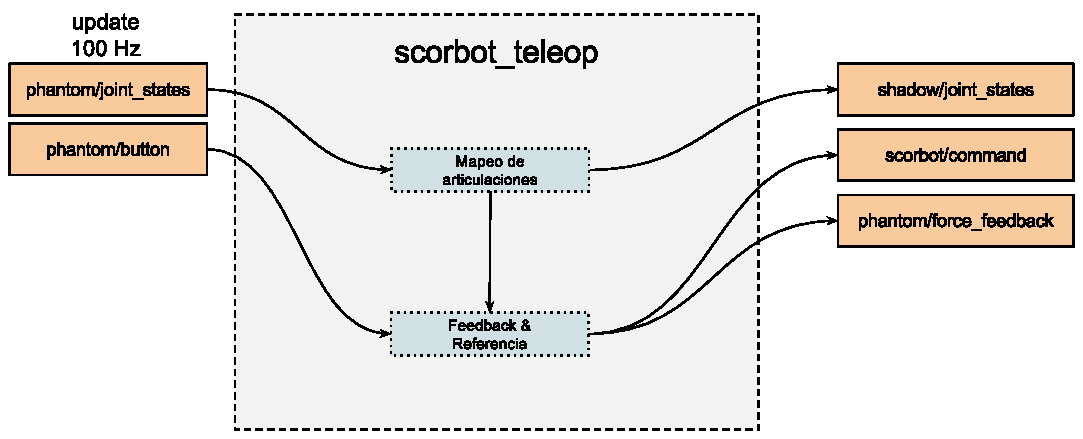
\includegraphics[width=0.8\textwidth]{img/cap4/scorbot_teleop.pdf}
  \caption{Diagrama del nodo \texttt{scorbot\_teleop}.}
  \label{cap4_scorbot_teleop}
\end{figure}

La función utilizada para el mapeo entre los \textit{joints} del Phantom Omni y el robot Scorbot sigue la linea planteada en \cite{david}, donde se considera un \textit{workspace} (espacio de trabajo) proporcional. De esta forma, la función lineal presentada en la Ecuación \ref{cap4_scorbot_mapping} realiza el mapeo planteado.

\begin{equation}\label{cap4_scorbot_mapping}
{\theta_S}_{i} = ({\theta_P}_{i} - {\Theta_{P-}}_{i}) \left(  \frac{{\Theta_{S+}}_{i} - {\Theta_{S-}}_{i}}{{\Theta_{P+}}_{i} - {\Theta_{P-}}_{i}}   \right) + {\Theta_{S-}}_{i} + H_i \, \mbox{con } i \in {1, \dots, 5}
\end{equation}

Donde ${\Theta_{P+}}_i$ y ${\Theta_{P-}}_i$ corresponde a los limites fisicos de la articulación $i$-ésima del Phantom Omni, los limites de las articulaciones del robot Scorbot siguen la misma notación ${\Theta_{S+}}_i$ y ${\Theta_{S-}}_i$, ${\theta_P}_{i}$ es la posición actual de la articulación $i$-ésima del Phantom Omni y ${\theta_S}_{i}$ la del robot Scorbot. Notar que la constante de proporcionalidad corresponde a la relación entre los rangos de movimiento, esto asegura que el robot Scorbot y el Phantom tienen un rango de actuación completo. La constante $H_i$ permite añadir una compensación para que la posición \textit{home} de ambos dispositivos.

La Figura \ref{cap4_scorbot_teleop} muestra funcinamiento interno del nodo \texttt{scorbot\_teleop}, el mapeo entre el Phantom y el Scorbot \textit{shadow} se realiza de forma continua con propósitos de visualización. La retroalimentación hápica es calculada a partir de la differencia en la posición del Scorbot \textit{shadow} y el robot real, dado que ambos dispositivos tienen una morfología similar y poseen el mismo número de grados de libertad, el cálculo se realiza la ley de Hooke \cite{handbook}, donde la posición corresponde a la posición de las articulaciones, como se indica en la Ecuación \ref{cap4_hooke}.

\begin{equation}\label{cap4_hooke}
F_i = K_i({\theta_{shadow}}_i - {\theta_{scorbot}}_i) \, \mbox{con } i \in {1,2,3}
\end{equation}

Donde $K_i > 0 \, \mbox{con } i \in {1,2,3}$. Notamos que el cálculo solo considera en las primeras tres articulaciones, pues el Phantom Omni solo posee tres articulaciones actuadas. En el robot Scorbot, las últimas dos articulaciones se encuentran cercanas al efector y definen su orientación, por lo que son las tres primeras articulaciones las que tinen el rol principal en definir la posición del efector.

\subsubsection{Visualización}

La visualización principal se realizó en el software \texttt{rviz}, ahí se añadió el modelo del robot principal y \texttt{scorbot\_shadow}, que representa la posición de referencia del robot Scorbot, como se ve en la Figura \ref{cap4_scorbot_shadow}.

\begin{figure}[H]
  \centering
  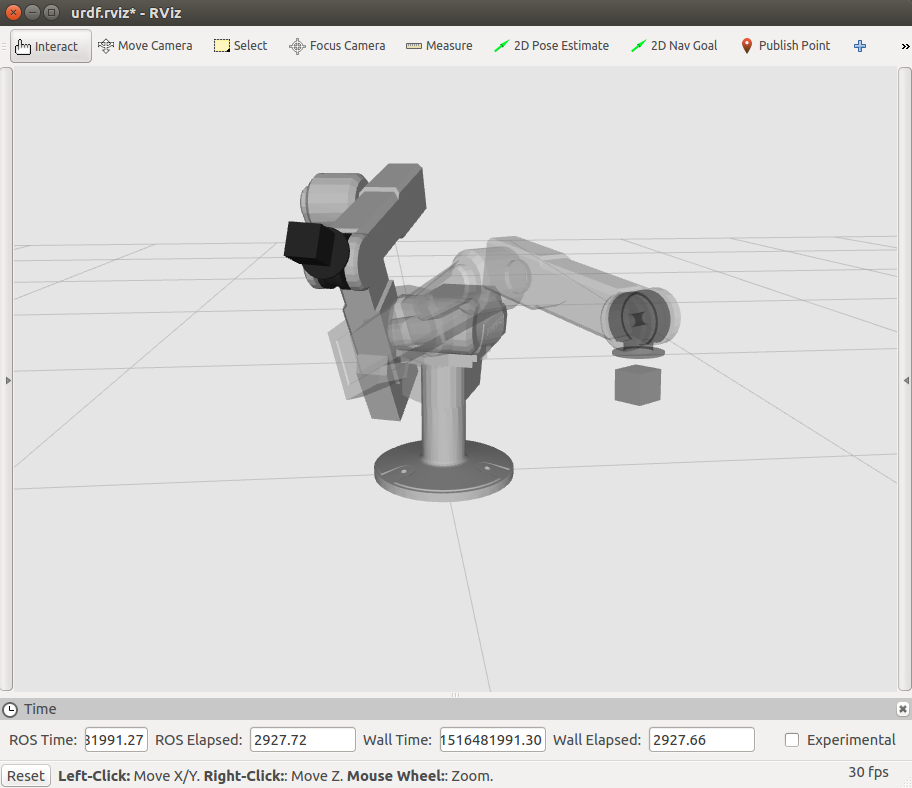
\includegraphics[width=0.6\textwidth]{img/cap4/scorbot_shadow.png}
  \caption{Applicación con el modelo real y \textit{shadow} en \textit{RViz}.}
  \label{cap4_scorbot_shadow}
\end{figure}

Como se describió en la Sección \ref{cap4_teleoperacion}, el nodo \texttt{scorbot\_teleop} es el nodo encargado de publicar el estado del \texttt{scorbot\_shadow}, por otro lado, \textit{driver} publica el estado del robot Scorbot. Gracias al nodo \texttt{robot\_state\_publisher} se obtiene la \textit{pose} de cada \textit{link} en el espacio, información que es publicada en el tópico \texttt{\textbackslash tf}. La Figura \ref{cap4_tf}, muestra la estructura de las distintas transformadas de coordenas del sistema, para la correcta visualización se ha puesto que ambos robots tengan la misma base. 

\begin{figure}[H]
  \centering
  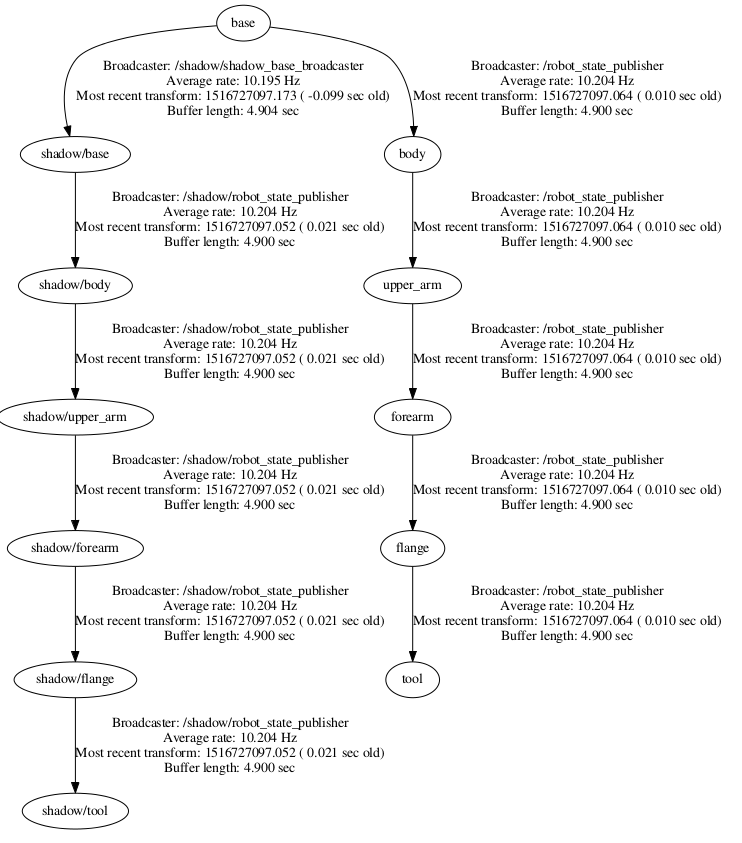
\includegraphics[width=0.6\textwidth]{img/cap4/tf.png}
  \caption{Estructura de transformadas del sistema.}
  \label{cap4_tf}
\end{figure}






